\section{Background}
\begin{frame}
    \frametitle{Background}
    \framesubtitle{Table of Contents}
    {
        \hypersetup{hidelinks}
        \tableofcontents[currentsection, hideothersubsections]
    }
\end{frame}

\subsection{Steps of MTMCT}
\begin{frame}
    \frametitle{Background}
    \framesubtitle{Steps of MTMCT}

    \begin{figure}[ht]
        \centering
        \begin{tikzpicture}[node distance=1.5cm and 0.5cm, auto]
    % Place nodes
    \node [block] (detection) {Detection};
    \node [block, right=of detection] (feature) {Feature Extraction};
    \node [block, right=of feature] (association) {Data Association};
    \node [block, right=of association] (tracking) {Tracking};

    % Draw edges
    \draw [arrow] (detection) -- (feature);
    \draw [arrow] (feature) -- (association);
    \draw [arrow] (association) -- (tracking);
\end{tikzpicture}
        \caption{Steps of an MTMCT System}\label{fig:mtmct_steps}
    \end{figure}

    \begin{itemize}
        \item <2->\textbf{Detection:} Detect objects in each frame of each camera
              \vspace{5pt}
        \item <3->\textbf{Feature Extraction:} Extract features from each detection
              \vspace{5pt}
        \item <4->\textbf{Data Association:} Associate detections with existing trajectories
              \begin{itemize}
                  \item \textbf{Intra-Camera:} Within each camera
                  \item \textbf{Inter-Camera:} Across cameras
              \end{itemize}
              \vspace{5pt}
        \item <5->\textbf{Tracking:} Maintaining trajectories over time\\(create, update, delete)
    \end{itemize}
\end{frame}

\subsection{Intra- vs.~Inter-Camera Tracking}
\begin{frame}
    \frametitle{Background}
    \framesubtitle{Intra- vs.~Inter-Camera Tracking}

    \begin{figure}[ht]
        \centering
        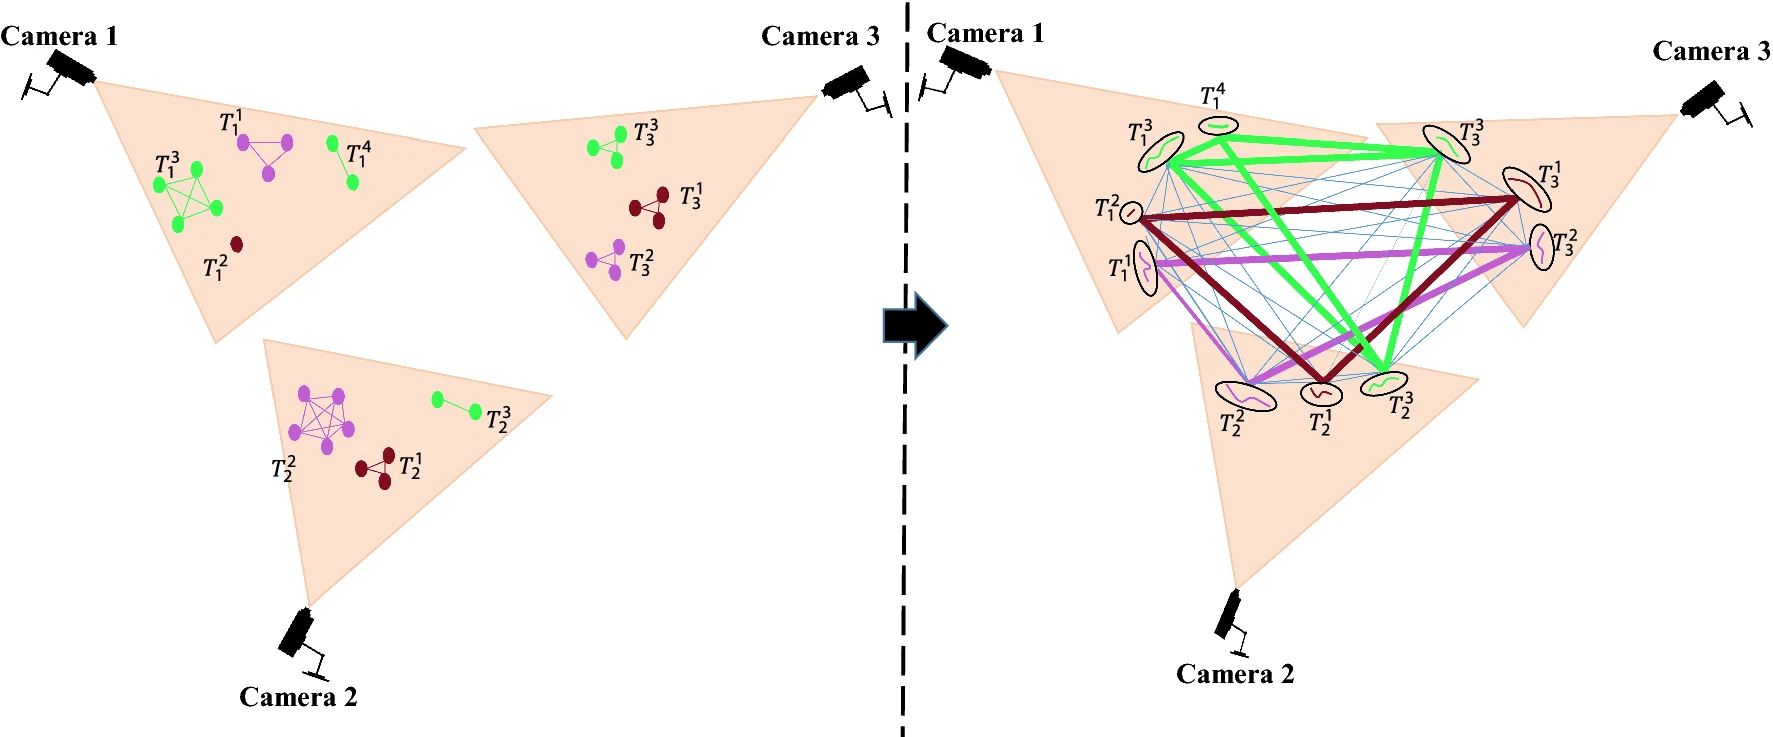
\includegraphics[width=0.75\textwidth]{resources/fig/Tesfaye19-intra_inter_camera_tracking.png}
        \caption[Intra- and Inter-Camera Tracking]{Intra- (left) and Inter-Camera (right) Tracking~\cite[Fig.~1]{Tesfaye19}}\label{fig:intra_inter_camera_tracking}
    \end{figure}
\end{frame}

\subsection{Tracking Process}
\begin{frame}
    \frametitle{Background}
    \framesubtitle{Tracking Process}

    \begin{figure}[ht]
        \centering
        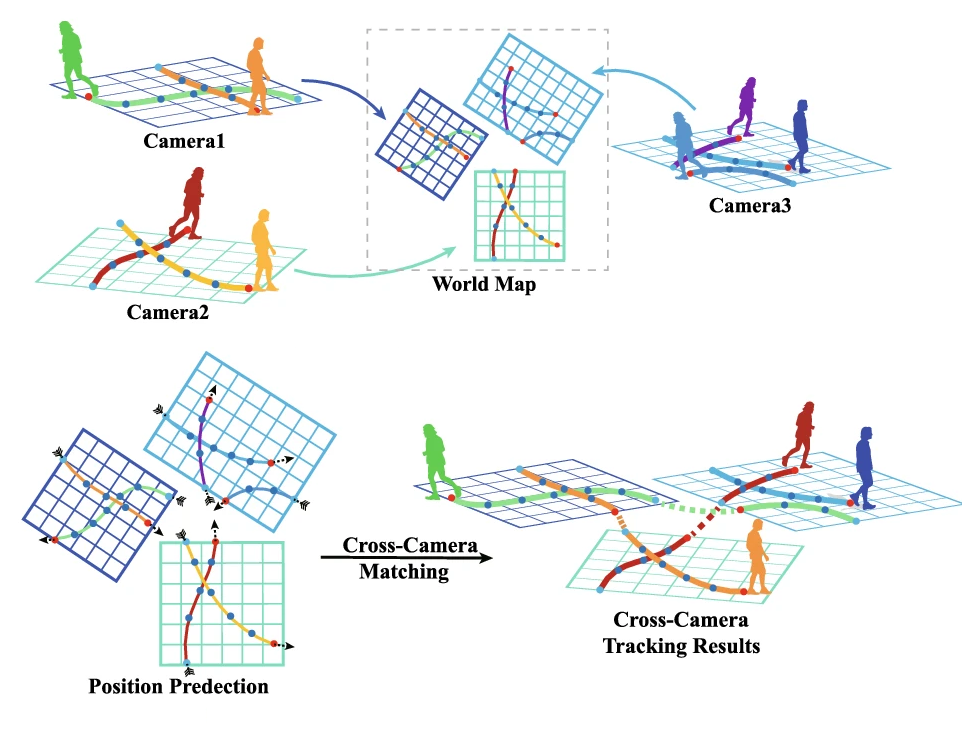
\includegraphics[width=0.75\textwidth]{resources/fig/Ma21-tracking_process.png}
        \caption[Tracking Process]{Tracking Process~\cite[Fig.~1]{Ma21}}\label{fig:projection}
    \end{figure}
\end{frame}

\subsection{Fundamental Concepts}
\begin{frame}
    \frametitle{Background}
    \framesubtitle{Fundamental Concepts}

    \begin{itemize}
        \item <1->Single-Target Single-Camera Tracking (STSCT)
              \begin{itemize}
                  \item Simplest form of tracking
                  \item Track a single target in FOV of a single camera
                  \item \textbf{Goal:} Maintain ID and trajectory of target
              \end{itemize}
              \vspace{5pt}
        \item <2->Multi-Target Single-Camera Tracking (MTSCT)
              \begin{itemize}
                  \item Builds on principles of STSCT
                  \item Adds complexity of multiple targets
                  \item \textbf{Goal:} Maintain IDs and trajectories of targets, avoid ID switches
              \end{itemize}
    \end{itemize}
\end{frame}

\subsection{Challenges in MTMCT}
\begin{frame}
    \frametitle{Background}
    \framesubtitle{Challenges in MTMCT}

    \begin{itemize}
        \item <1->\textbf{Occlusions:} Targets can be occluded by other targets or objects
              \vspace{5pt}
        \item <2->\textbf{Varying Lighting Conditions:} Lighting conditions can change over time and across cameras
              \vspace{5pt}
        \item <3->\textbf{Camera Specifications:} Cameras can have different specifications (e.g.~resolution, FPS, FOV, angle, ...)
              \vspace{5pt}
        \item <4->\textbf{Uncertainties (unknown number of):}
              \begin{itemize}
                  \item Targets in entire camera
                  \item Targets in single camera
                  \item Cameras a tracked target appears
              \end{itemize}
    \end{itemize}
\end{frame}

\subsection{Metrics and Evaluation}
\begin{frame}
    \frametitle{Background}
    \framesubtitle{Metrics and Evaluation}

    \begin{itemize}
        \item <1->\textbf{MOTP:} Multiple Object Tracking Precision\\(accuracy of object localization)~\cite{Bernardin08}
              \vspace{0pt}
        \item <1->\textbf{MOTA:} Multiple Object Tracking Accuracy\\(three in one: misses, false positives, ID switches)~\cite{Bernardin08}
              \vspace{5pt}
        \item <2->\textbf{IDF1:} ID F1 Score (harmonic mean of precision and recall)~\cite{Ristani16}
              \vspace{5pt}
        \item <3->\textbf{MT:} Mostly Tracked (\(\geq80\%\) correctly tracked)~\cite{Wu06}
              \vspace{0pt}
        \item <3->\textbf{ML:} Mostly Lost (\(\leq20\%\) correctly tracked)~\cite{Wu06}
              \vspace{5pt}
              \begin{figure}[ht]
                  \centering
                  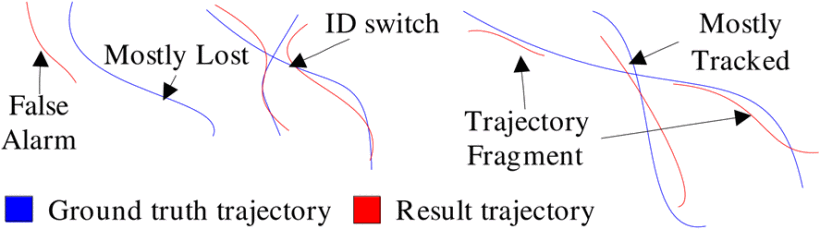
\includegraphics[width=0.75\textwidth]{resources/fig/Wu06-MT_ML.png}
                  \caption[MT and ML]{MT and ML~\cite[source image:][Fig.~5]{Wu06}}\label{fig:mt_ml}
              \end{figure}
    \end{itemize}
\end{frame}